\documentclass[11pt,reqno]{amsart}
\usepackage{amsfonts,amsmath,amssymb,amsbsy,amstext,amsthm,mathtools}
\usepackage{accents,color,enumerate,enumitem,float,fullpage,verbatim}

\usepackage[margin=1.0049in,includeheadfoot]{geometry}

\usepackage{url}
%\usepackage[colorlinks=true,hyperindex, linkcolor=magenta, pagebackref=false, citecolor=cyan,draft]{hyperref}
\usepackage[nolinks=true]{hyperref}

%\usepackage[alphabetic]{amsrefs} 

%\usepackage{eucal,bm,kpfonts,mathbbol}
\usepackage[dvipsnames]{xcolor}

\usepackage{tikz,tikz-cd}	
\usetikzlibrary{positioning, matrix, shapes}         								    				
\usetikzlibrary{arrows,calc,matrix}

\usepackage{lscape}

\usepackage{microtype}


\usepackage{titlesec}		
\setcounter{secnumdepth}{4}						     					% Allows one to use nice section titles
\titleformat{\section}[block]{\scshape\bfseries\filcenter}{\thesection.}{1em}{}		% Creates section titles
\titleformat{\subsection}[runin]{\scshape\bfseries}{\thesubsection}{1em}{}			% Creates subsection titles
\titleformat{\subsubsection}[runin]{\scshape\bfseries}{\thesubsubsection}{1em}{}			% Creates subsection titles

\usepackage[titles]{tocloft}								     					% Creates table of fancy contents
\setcounter{tocdepth}{4}
\renewcommand{\contentsname}{}	     					% Renames and centers title of ToC

\usepackage{multirow}
\usepackage{array}
\usepackage{booktabs}
\newcolumntype{M}[1]{>{\centering\arraybackslash}m{#1}}
\newcolumntype{N}{@{}m{0pt}@{}}
\usepackage{diagbox}
\usepackage{cancel}

\newtheorem{lemma}{Lemma}[section]
\newtheorem{theorem}[lemma]{Theorem}
\newtheorem{goalTheorem}[lemma]{Goal Theorem}
\newtheorem{problem}[lemma]{Research Problem}
\newtheorem{prop}[lemma]{Proposition}
\newtheorem{cor}[lemma]{Corollary}
\newtheorem{conj}[lemma]{Conjecture}
\newtheorem{claim}[lemma]{Claim}
\newtheorem{defn}[lemma]{Definition} 
\newtheorem{notation}[lemma]{Notation} 
\newtheorem{exercise}[lemma]{Exercise}
\newtheorem{question}[lemma]{Question}
\newtheorem*{assumption}{Assumption}
\newtheorem{principle}[lemma]{Principle}
\newtheorem{heuristic}[lemma]{Heuristic}

\newtheorem{theoremalpha}{Theorem}
\newtheorem{corollaryalpha}[theoremalpha]{Corollary}
\renewcommand{\thetheoremalpha}{\Alph{theoremalpha}}

\theoremstyle{remark}
\newtheorem{remark}[lemma]{Remark}
\newtheorem{example}[lemma]{Example}
\newtheorem{cexample}[lemma]{Counterexample}

% Commands
\newcommand{\initial}{\operatorname{in}}
\newcommand{\NF}{\operatorname{NF}}
\newcommand{\HF}{\operatorname{HF}}
\newcommand{\Hilb}{\operatorname{Hilb}}
\newcommand{\depth}{\operatorname{depth}}
\newcommand{\reg}{\operatorname{reg}}
\newcommand{\Span}{\operatorname{span}}
\newcommand{\img}{\operatorname{img}}
\newcommand{\inn}{\operatorname{in}}

\newcommand{\length}{\operatorname{length}}
\newcommand{\coker}{\operatorname{coker}}
\newcommand{\adeg}{\operatorname{adeg}}
\newcommand{\pdim}{\operatorname{pdim}}
\newcommand{\Spec}{\operatorname{Spec}}
\newcommand{\Ext}{\operatorname{Ext}}
\newcommand{\Tor}{\operatorname{Tor}}
\newcommand{\LT}{\operatorname{LT}}
\newcommand{\im}{\operatorname{im}}
\newcommand{\NS}{\operatorname{NS}}
\newcommand{\Frac}{\operatorname{Frac}}
\newcommand{\Khar}{\operatorname{char}}
\newcommand{\Proj}{\operatorname{Proj}}
\newcommand{\id}{\operatorname{id}}
\newcommand{\Div}{\operatorname{Div}}
\newcommand{\Kl}{\operatorname{Cl}}
\newcommand{\tr}{\operatorname{tr}}
\newcommand{\Tr}{\operatorname{Tr}}
\newcommand{\Supp}{\operatorname{Supp}}
\newcommand{\ann}{\operatorname{ann}}
\newcommand{\Gal}{\operatorname{Gal}}
\newcommand{\Pic}{\operatorname{Pic}}
\newcommand{\QQbar}{{\overline{\mathbb Q}}}
\newcommand{\Br}{\operatorname{Br}}
\newcommand{\Bl}{\operatorname{Bl}}
\newcommand{\Kox}{\operatorname{Cox}}
\newcommand{\conv}{\operatorname{conv}}
\newcommand{\getsr}{\operatorname{Tor}}
\newcommand{\diam}{\operatorname{diam}}
\newcommand{\Hom}{\operatorname{Hom}} %done
\newcommand{\sheafHom}{\mathcal{H}om}
\newcommand{\Gr}{\operatorname{Gr}}
\newcommand{\rank}{\operatorname{rank}} 
\newcommand{\codim}{\operatorname{codim}}
\newcommand{\Sym}{\operatorname{Sym}} %done
\newcommand{\GL}{{GL}}
\newcommand{\Prob}{\operatorname{Prob}}
\newcommand{\Density}{\operatorname{Density}}
\newcommand{\Syz}{\operatorname{Syz}}
\newcommand{\pd}{\operatorname{pd}}
\newcommand{\supp}{\operatorname{supp}}
\newcommand{\cone}{\operatorname{\textbf{cone}}}
\newcommand{\Res}{\operatorname{Res}}
\newcommand{\HS}{\operatorname{HS}}
\newcommand{\Cl}{\operatorname{Cl}}
\newcommand{\oO}{\operatorname{O}}

\newcommand{\defi}[1]{\textsf{#1}} % for defined terms

\newcommand{\remd}{\operatorname{remd}}
\newcommand{\colim}{\operatorname{colim}}
\newcommand{\trideg}{\operatorname{tri.deg}}
\newcommand{\indeg}{\operatorname{index.deg}}
\newcommand{\moddeg}{\operatorname{mod.deg}}
\newcommand{\Desc}{\operatorname{Desc}}
\newcommand{\inter}{\operatorname{int}}
\newcommand{\Nef}{\operatorname{Nef}}
\newcommand{\Jac}{\operatorname{Jac}}
\newcommand{\Cox}{\operatorname{Cox}}
\newcommand{\gon}{\operatorname{gon}}
\newcommand{\cliff}{\operatorname{Cliff}}

\newcommand{\doot}{\bullet}

\newcommand{\Alt}{\bigwedge\nolimits}
\newcommand{\Set}{\text{\bf Set}}										% Category of Sets
\newcommand{\Sch}{\text{\bf Sch}}										% Category of Abelian Groups
\newcommand{\Mod}[1]{\ (\mathrm{mod}\ #1)}




%%%%%%%%%%%%%%%%%%%%%%%%%%%%%% Letters  %%%%%%%%%%%%%%%%%%%%%%%%%%%%%%%%%%%%%%%%%%%%
%%%%%%%%%%%%%%%%%%%%%%%%%%%%%%%%%%%%%%%%%%%%%%%%%%%%%%%%%%%%%%%%%%%%%%%%%%%%%%
\renewcommand{\aa}{\mathbf{a}}
\newcommand{\dd}{\mathbf{d}}
\newcommand{\nn}{\mathbf{n}}
\newcommand{\ee}{\mathbf{e}}
\newcommand{\ff}{\mathbf{f}}
\newcommand{\vv}{\mathbf{v}}
\newcommand{\ww}{\mathbf{w}}
\newcommand{\one}{\mathbf{1}}
\newcommand{\pp}{\mathbf{p}}
\newcommand{\qq}{\mathbf{q}}

\renewcommand{\AA}{\mathbb{A}}
\newcommand{\BB}{\mathbb{B}}
\newcommand{\CC}{\mathbb{C}}
\newcommand{\DD}{\mathbb{D}}
\newcommand{\EE}{\mathbb{E}}
\newcommand{\FF}{\mathbb{F}}
\newcommand{\GG}{\mathbb{G}}
\newcommand{\HH}{\mathbb{H}}
\newcommand{\II}{\mathbb{I}}
\newcommand{\JJ}{\mathbb{J}}
\newcommand{\KK}{\mathbb{K}}
\newcommand{\LL}{\mathbb{L}}
\newcommand{\MM}{\mathbb{M}}
\newcommand{\NN}{\mathbb{N}}
\newcommand{\PP}{\mathbb{P}}
\newcommand{\QQ}{\mathbb{Q}}
\newcommand{\RR}{\mathbb{R}}
\renewcommand{\SS}{\mathbb{S}}
\newcommand{\TT}{\mathbb{T}}
\newcommand{\UU}{\mathbb{U}}
\newcommand{\VV}{\mathbb{V}}
\newcommand{\WW}{\mathbb{W}}
\newcommand{\XX}{\mathbb{X}}
\newcommand{\YY}{\mathbb{Y}}
\newcommand{\ZZ}{\mathbb{Z}}


\newcommand{\cA}{\mathcal{A}}
\newcommand{\cB}{\mathcal{B}}
\newcommand{\cC}{\mathcal{C}}
\newcommand{\cD}{\mathcal{D}}
\newcommand{\cE}{\mathcal{E}}
\newcommand{\cF}{\mathcal{F}}
\newcommand{\cG}{\mathcal{G}}
\newcommand{\cH}{\mathcal{H}}
\newcommand{\cI}{\mathcal{I}}
\newcommand{\cJ}{\mathcal{J}}
\newcommand{\cK}{\mathcal{K}}
\newcommand{\cL}{\mathcal{L}}
\newcommand{\cM}{\mathcal{M}}
\newcommand{\cN}{\mathcal{N}}
\newcommand{\cO}{\mathcal{O}}
\newcommand{\cP}{\mathcal{P}}
\newcommand{\cQ}{\mathcal{Q}}
\newcommand{\cR}{\mathcal{R}}
\newcommand{\cS}{\mathcal{S}}
\newcommand{\cT}{\mathcal{T}}
\newcommand{\cU}{\mathcal{U}}
\newcommand{\cV}{\mathcal{V}}
\newcommand{\cW}{\mathcal{W}}
\newcommand{\cX}{\mathcal{X}}
\newcommand{\cY}{\mathcal{Y}}
\newcommand{\cZ}{\mathcal{Z}}

\DeclareMathOperator{\RB}{RB}
\DeclareMathOperator{\Trop}{Trop}
\DeclareMathOperator{\trop}{Trop}

\DeclareMathOperator{\OO}{O}
\DeclareMathOperator{\SL}{SL}
\DeclareMathOperator{\Sp}{Sp}
\DeclareMathOperator{\Ag}{\mathcal{A}_{g}}
\DeclareMathOperator{\PDrt}{PD^{rt}}
\DeclareMathOperator{\PD}{PD}
\DeclareMathOperator{\Herm}{Herm}

\newcommand{\juliette}[1]{{\color{red} \sf $\spadesuit\spadesuit\spadesuit$ Juliette: [#1]}}

\newcommand{\kit}[1]{{\color{blue} \sf Kit: [#1]}}
\newcommand{\jcite}{{\color{blue} \sf $\heartsuit\heartsuit\heartsuit$:cite}}

\title{Project Description: Multigraded Homological Algebra and Geometry}

%\author{Juliette Bruce}
%\address{Department of Mathematics, University of Wisconsin, Madison, WI}
%\email{\href{mailto:juliette.bruce@math.wisc.edu}{juliette.bruce@math.wisc.edu}}
%\urladdr{\url{http://math.wisc.edu/~juliettebruce/}}

%\thanks{The author was partially supported by the NSF GRFP under Grant No. DGE-1256259 and NSF grant DMS-1502553.}

%\subjclass[2010]{13D02, 14M25}

\begin{document} 
\thispagestyle{empty}
\pagestyle{empty}
%\maketitle
\begingroup  
  \centering
  \large\scshape\bfseries Project Description: Tropicalizations of Shimura Varieties\\[1em]
\endgroup

%\tableofcontents

\setcounter{section}{0}

\noindent This proposal involves research in algebraic geometry and commutative algebra with several connections to computation and combinatorics, as well as a wide array of broader impacts.
% Additionally, it includes a wide array of broader impacts. As an overview: 
\begin{itemize}[leftmargin=*]
	\item \S~\ref{sec:prior-work} \textbf{Results of Prior NSF Support.} 
	\item \S~\ref{sec:trop-moduli} \textbf{Tropicalizations of Shimura Varieties}
	\item \S~\ref{sec:gen-trop} \textbf{A General Theory of Tropical Shimura Varieties}
	\item \S~\ref{sec:trop-mod} \textbf{Tropical Modular Interpretations}
	\item \S~\ref{sec:computing} \textbf{Computing Weight Zero Compactly Supported Cohomology of Shimura Varieties}
	\item \S~\ref{sec:alg-structure} \textbf{Algebraic Structures on the Weight Zero Cohomology of Shimura Varieties}
%	\item By developing tools in multigraded commutative algebra, like analogs of lex ideals and generalizations of Macaulay's theorem, this project looks to characterize when mutligraded Hilbert schemes are non-empty, connected, or smooth.  
%	By developing tools in multigraded commutative algebra, like analogs of lex ideals and generalizations of Macaulay's theorem,
	\item \S~\ref{sec:broader-impacts} \textbf{Broader Impacts.}
\end{itemize}

\section{Results of Prior NSF Support}\label{sec:prior-work}

During 2020-2022 the PI was supported by an NSF Postdoctoral Research Fellowship (NSF Grant No. MSPRF DMS-2002239, \$150,000) titled \textit{Asymptotic Syzygies in Algebraic Geometry}. In this period the PI made major contributions to extending our understanding of homological algebra on toric varieties (see Section~\ref{subsec:prior:homological-algebra-on-toric}) and the cohomology of moduli spaces (see Section~\ref{subsec:prior:cohomology-of-ag}). These works resulted in 5 new papers being posted to the arXiv \cite{BCEGLY22,bruceHellerSayrafi21,bruceHellerSayrafi22,brandtBruceCorey23,BBCMMW24}.

During 2015-2020 the PI was supported by an NSF Graduate Research Fellowship (NSF Grant No. DGE-1256259, \$150,000) title \textit{Syzygies in Algebraic Geometry}. In this period the PI made substantial contributions to commutative algebra and algebraic geometry, including furthering our understanding of syzygies on higher dimensional varieties and extending classical results in algebraic geometry and commutative algebra to finite fields. This resulted in the PI posting 8 new papers to the arXiv \cite{ABLS20,BBBKR17,bruceErman19,bruceLi20,BEGY20,BEGY21,bruce24,bruce22}.

Additionally, of the 12 new papers the PI posted to the arXiv during these periods of support 9 of these above-mentioned papers were accepted for publication, including in such journals as \textit{Algebra \& Number Theory} \cite{bruceErman19}, \textit{Geometry \& Topology} \cite{BBCMMW24}, \textit{Journal of Algebra} \cite{BCEGLY22}, and \textit{Experimental Mathematics} \cite{BEGY20}. The PI contributed to 4 open-source software packages, one public-facing database, and two articles for the \textit{Notices of the AMS} \cite{BBB21,bruceNotices22}. All of these are available via the software \textit{Macaulay2} or the PI's website and Github. A more detailed summary of these results and their intellectual merits continues in the following sections. 

\subsection{Homological Algebra on Toric Varieties}\label{subsec:prior:homological-algebra-on-toric}


Introduced by Mumford, the Castelnuovo–Mumford Regularity of a projective variety $X\subset \PP^{r}$ is a measure of the complexity of $X$ given in terms of the vanishing of certain cohomology groups of $X$. Roughly speaking one should think about Castelnuovo--Mumford regularity as being a numerical measure of geometric complexity. Mumford was interested in such a measure as it plays a key role in constructing Hilbert and Quot schemes. In particular, being $d$-regular implies that $\cF(d)$ is globally generated. However, Eisenbud and Goto showed that regularity is also closely connected to interesting homological properties.

\begin{theorem}\cite{eisenbudGoto84}\label{thm:eisenbud-goto}
Let $\cF$ be a coherent sheaf on $\PP^{r}$ and $M=\bigoplus_{e\in\ZZ} H^0(\PP^{r},\cF(e))$ the corresponding section ring. The following are equivalent: (1) $M$ is $d$-regular; (2) $\beta_{p,q}(M)=0$ for all $p\geq0$ and $q>d+i$; (3) $M_{\geq d}$ has a linear resolution. 
\end{theorem}

Maclagan and Smith introduced multigraded Castelnuovo--Mumford regularity, where $\PP^{r}$ can be replaced by any toric variety. Similarly to the definition in the classical setting multigraded Castelnuovo--Mumford regularity is defined in terms of the vanishing of cohomology groups, however, the multigraded Castelnuovo--Mumford regularity of a subvariety or module is not a single number, but an infinite subset of $\ZZ^{r}$. As an example, let us consider the case of products of projective spaces. Fixing a dimension vector $\nn=(n_1,n_2,\ldots,n_{r})\in \NN^{r}$ we let $\PP^{\nn}\coloneqq \PP^{n_1}\times \PP^{n_2}\times \cdots \times \PP^{n_r}$ and $S=\KK[x_{i,j} \; |\; 1\leq i \leq r, 0\leq j \leq n_{i}]$ be the Cox ring of $\PP^{\nn}$ with the $\Pic(X)\cong \ZZ^{r}$-grading given by $\deg x_{i,j} = \ee_{i} \in \ZZ^{r}$, where $\ee_{i}$ is the $i$-th standard basis vector in $\ZZ^{r}$. Fixing some notation given $\dd\in \ZZ^{r}$ and $i\in \ZZ_{\geq0}$ we let $L_{i}(\dd)\coloneqq \bigcup_{\substack{\vv \in \NN, |\vv| = i}} (\dd-\vv)+\NN^{r}$. Note when $r=2$ the region $L_{i}(\dd)$ looks like a staircase with $(i+1)$-corners. Roughly speaking we define regularity by requiring the $i$-th cohomology of certain twists of $\cF$ to vanish on $L_{i}$. 

\begin{defn}\cite[Definition 6.1]{maclaganSmith04}\label{def:mg-reg}
A coherent sheaf $\cF$ on $\PP^{\nn}$ is $\dd$-regular if and only if $H^i\left(\PP^{\nn}, \cF(\ee)\right) =0$ for all $\ee\in L_{i}(\dd)$. The multigraded Castelnuovo--Mumford regularity of $\cF$ is then the set: 
\[
\reg(\cF) \coloneqq \left \{ \dd\in \ZZ^{r} \;\; \big| \;\; \text{$\cF$ is $\dd$-regular}\right\}\subset \ZZ^{r}.
\]
\end{defn}


The obvious approaches to generalize Theorem~\ref{thm:eisenbud-goto} to a product of projective spaces turn out not to work. For example, the multigraded Betti numbers do not determine multigraded Castelnuovo--Mumford regularity \cite[Example 5.1]{bruceHellerSayrafi21} Despite this we show that part (3) of Theorem~\ref{thm:eisenbud-goto} can be generalized. To do so we introduce the following generalization of linear resolutions. 

\begin{defn}
A complex $F_{\bullet}$ of $\ZZ^{r}$-graded free $S$-modules is $\dd$-quasilinear if and only if $F_{0}$ is generated in degree $\dd$ and each twist of $F_{i}$ is contained in $L_{i-1}(\dd-\one)$.
\end{defn}

\begin{theorem}\cite[Theorem A]{bruceHellerSayrafi21}\label{thm:mgreg-main}
Let $M$ be a (saturated) finitely generated $\ZZ^{r}$-graded $S$-module:
\[
\text{$M$ is $\dd$-regular} \iff  \text{$M_{\geq\dd}$ has a $\dd$-quasilinear resolution}.
\]
\end{theorem}

The proof of Theorem~\ref{thm:mgreg-main} is based in part on a spectral sequence argument that relates the Betti numbers of $M_{\geq\dd}$ to the Fourier--Mukai transform of $\widetilde{M}$ with Beilinson's resolution of the diagonal as the kernel.  Recent breakthroughs \cite{HHL23, brownErman23-2} understanding resolutions of the diagonal on arbitrary toric varieties mean that there is hope one may be able to generalize the above argument to arbitrary toric varieties. With this in mind, I am interested in pursuing the following question

Building upon our work discussed above -- and inspired by previous work on $\PP^{r}$ \cite{BEL91,CHT99,Kodiyalam00} -- my collaborators and I also studied the asymptotic regularity of powers of ideals on arbitrary toric varieties. In particular, Definition~\ref{def:mg-reg} can be extended to all toric varieties by letting $S$ be Cox ring of the toric variety $X$, replacing $\ZZ^r$ with the Picard group of $X$, and replacing $\NN^{r}$ with the nef cone of $X$. My collaborators and I show that the multigraded regularity of powers of ideals is bounded and translates in a predictable way. In particular, the regularity of $I^{t}$ essentially translates within $\Nef X$ in fixed directions at a linear rate.
 

\begin{theorem}\cite[Theorem 4.1]{bruceHellerSayrafi22}
  There exists a degree $\aa\in\Pic X$, depending only on $I$, such that for each integer $t>0$ and each pair of degrees $\qq_1,\qq_2\in\Pic X$ satisfying $\qq_1\geq\deg f_i\geq\qq_2$ for all generators $f_i$ of $I$, we have
	\[ t\qq_1+\aa+\reg S \subseteq \reg\!\left(I^t\right) \subseteq t\qq_2+\Nef X. \]
\end{theorem}

\subsection{Top-Weight Cohomology of $\mathcal{A}_{g}$}\label{subsec:prior:cohomology-of-ag}

The moduli space of (principally polarized) abelian varieties of dimension $g$, is a smooth variety $\cA_{g}$ (truthfully a smooth Delinge--Mumford stack) whose points are in one to one correspondence with isomorphism classes of principally polarized abelian varieties of dimension $g$. Concretely, we may view it as the quotient $[\mathbb{H}_g/\mathrm{Sp}(2g, \ZZ)]$ where $\HH_{g}$ is the Siegel upper half-space. Notice this means that $\cA_{g}$  is a rational classifying space for the integral symplectic group $\mathrm{Sp}(2g,\ZZ)$. Similar to the moduli space of curves $\cA_{g}$ has long been studied, but much remains unknown about its geometry. For example, the (singular) cohomology is $\cA_{g}$ is only fully known for $g\leq 4$, with $g=0,1$ being relatively easy, $g=2$ which is a classical result of Igusa \cite{igusa62},  $g=3$ due to work of Hain \cite{hain02}, and $g=4$ being deducible from \cite{HT12,HT18}. In fact until recent work by myself and co-authors it was unknown whether $H^{2k+1}(\cA_{g};\QQ)\neq0$ for some $g$ and $k$. This was a question posed by Grushevsky. that my recent work answered \cite{grushevsky09}. 

Building upon the work of Chan, Galatius, and Payne, my co-authors and I developed new methods for understanding a certain canonical quotient of the cohomology of $\cA_{g}$. In particular, our results construct non-trivial cohomology classes in $H^{k}(\cA_{g}; \QQ)$ in a number of new cases. 

\begin{theorem}\cite[Theorem A]{BBCMMW24}\label{thm:Ag}
The rational cohomology $H^{k}\left(\cA_{g};\QQ\right)\neq0$ for:
\[
\text{$(g,k)=(5,15),(5,20),(6,30),(7,28),(7,33),(7,37)$, and $(7,42)$}.
\]
\end{theorem}

For broader context, since $\cA_g$ is a rational classifying space for $\mathrm{Sp}_{2g}(\ZZ)$ there is natural isomorphism $H^*(\cA_g;\QQ) \cong H^*(\mathrm{Sp}_{2g}(\ZZ);\QQ)$. In particular, the above results provide new non-vanishing results for $H^*(\mathrm{Sp}_{2g}(\ZZ);\QQ)$. However, my work takes advantage of the fact that since $\cA_g$  is a smooth and separated Deligne Mumford stack with a coarse moduli space which is an algebraic variety, permitting Deligne's mixed Hodge theory to be applied to study the rational cohomology of these groups. In particular, the rational cohomology of a %smooth 
complex algebraic variety $X$ of dimension $d$ admits a weight filtration with graded pieces $\Gr_{j}^W\!H^k(X;\mathbb{Q})$. %with $j$ ranging from %$k$ 
%$0$ to ${\rm min}\{2k, 2d\}$. 
As $\Gr_{j}^W\!H^k(X;\mathbb{Q})$ vanishes whenever $j>2d$, $\Gr_{2d}^W\!H^k(X;\mathbb{Q})$ is referred to as the {\em top-weight} part of $H^k(X;\QQ)$.)  In this way we deduce Theorem~\ref{thm:Ag} above as a corollary to computing the top-weight cohomology of $\cA_{g}$ for all $g\leq 7$.  


\subsection{Broader Impacts from Prior NSF Support}

\subsubsection{Organizing}\label{subsubsec:prior-organizing} I have organized 11 conferences: \textit{Math Careers Beyond Academia } (50 participants), \textit{M2@UW} (45 participants), \textit{Geometry and Arithmetic of Surfaces} (40 participants), \textit{Graduate Workshop in Commutative Algebra for Women \& Mathematicians of Other Minority Genders} (35 participants), \textit{CAZoom} (70 participants), \textit{Western Algebraic Geometry Symposium} (100 participants), \textit{GEMS of Combinatorics I \& II} (40 \& 30 participants), $\Spec(\overline{\QQ})$ (50 participants), \textit{BATMOBILE} (20 participants),  \textit{GEMS of Commutative Algebra} (40 participants). Additionally, I have organized three special sessions at AMS Sectional Meetings and the Joint Math Meetings. When organizing these conferences I have paid special attention to promoting women and other underrepresented groups in mathematics. For example, \textit{Graduate Workshop in Commutative Algebra for Women \& Mathematicians of Other Minority Genders} and \textit{GEMS in Combinatorics/Commutative Algebra}  focused on forming communities of women and non-binary researchers in commutative algebra and combinatorics. Further, $\Spec(\overline{\QQ})$ highlighted the research of LGBTQ+ mathematicians.


\subsubsection{Math Circles}
	From 2015 through 2018 I was heavily involved in the Madison Math Circle, including  2 years as the lead organizer. As an organizer, I worked to build stronger connections between the Madison Math Circle, local schools and teachers, and other outreach organizations focused on underrepresented groups. This led to weekly attendance to more than double. I also created a new outreach arm of the circle, which visits high schools around the state of Wisconsin to better serve students from underrepresented groups. This dramatically expanded the reach of the Madison Math Circle, and during my final year as an organizer, the circle reached over 300 students. While a post-doc at UC Berkeley I volunteered as a speaker with the Berkeley Math Circle. 

\subsubsection{Mentoring}
I have actively sought out ways to mentor undergraduate and graduate students, especially those from generally underrepresented groups. While a graduate student, I led reading courses with three undergraduates. One of these students, an undergraduate woman, worked with me for over a year, during which time I helped her apply for summer research projects. Working with \textit{Girls' Math Night Out} I lead two girls in high school through a project exploring cryptography. During 2018-2019, I mentored 6 first-year graduate students (all women or non-binary students). I also mentored two undergraduate women via the AWM's Mentoring Network. 

I advised two summer research projects for undergraduate students. The first of these projects ran virtually during Summer 2021 when 6 undergraduates worked on combinatorial questions related to my work in \cite{BBCMMW24}. In Summer 2022 I advised an undergraduate student on a research project related to my work on syzygies discussed in Section~\ref{subsec:prior:homological-algebra-on-toric}. This student is now a graduate student in mathematics and received an NSF GRF. As a postdoc, I began research projects with three graduate students (a majority of whom identify with a generally underrepresented group). These projects have resulted in two pre-prints, with additional projects still ongoing. Throughout the Spring and Summer of 2022, I did a reading course with a first-year graduate woman on algebraic geometry.

\subsubsection{Virtual Mathematics}
In response to the COVID-19 pandemic and the shift of many mathematical activities to virtual formats, I worked to find ways for these online activities to reach those often at the periphery. During Summer and Fall 2020, I helped with Ravi Vakil's \textit{Algebraic Geometry in the Time of Covid} project. This massive online open-access course in algebraic geometry brought together $\sim2,000$ participants from around the world. In Spring 2021, I organized an 8-week virtual reading course for undergraduates in algebraic geometry and commutative algebra. 

\subsubsection{A More Inclusive Community.} 
While a graduate student I co-founded oSTEM@UW as a resource for LGBTQ+ students in STEM, which eventually grew to over fifty active members. As one member said, ``It made me very happy to see other friendly LGBTQ+ faces around... Thanks so much for organizing this stuff -- it's really helpful''. From 2017-2020 I led the campus social organization for LGBTQ+ graduate and post-graduate students, which had over 350 members. 

Since Fall 2020 I have organized \textit{Trans Math Day}, an annual one-day virtual conference promoting the work of transgender and non-binary mathematicians. Highlighting the importance of such conferences one student participant said, ``I've been really considering leaving mathematics.  [Trans Math Day 2020] reminded me why I'm here and why I want to stay. ... If a conference like this had been around for me five years ago, my life would have been a lot better.'' Trans Math Day regularly has ~50 participants. 

During 2020-2023 I served as a board member for \textit{Spectra: The Association for LGBTQ+ Mathematicians}, including the inaugural president. I oversaw the growth and formalization of the organization, including the creation and adoption of bylaws, the creation of an invited lecture at the Joint Math Meetings, and a fundraising campaign that has raised over \$20,000.



\section{Tropicalizations of Shimura Varieties}\label{sec:trop-moduli}

While playing a central role in much of algebraic geometry, much remains unknown about the topology of many moduli spaces. For example, the rational cohomology of $\cM_{g}$, the moduli space of (smooth) genus $g$ curves, also known as the moduli space of compact Riemann surfaces of genus $g$ is only known for $g\leq 4$. This is despite the fact that classical results imply that $\cM_{g}$ should have a lot of cohomology because its Euler characteristic grows super exponentially. Recently, there has been substantial work utilizing combinatorial and tropical geometry to study many moduli spaces. Of particular note for this project is the work of Chan, Galatius, and Payne constructing new non-trivial cohomology classes, and showing that the dimension of certain cohomology groups of $\cM_{g}$ grow at least exponentially. 

\begin{theorem}\cite[Theorem 1.1]{CGP21}\label{thm:Mg}
For $g\geq2$ the dimension of $H^{4g-6}(\cM_{g};\QQ)$ grows at least exponentially. In particular $\dim H^{4g-6}\left(\cM_{g}; \QQ\right) > \beta^{g}$ for any real number $\beta<\beta_{0}$ where $\beta_{0}\approx1.3247\ldots$ is the real solution of $t^3-t-1=0$. 
\end{theorem}

Viewed from a (very) high level this result of Chan, Galatius, and Payne rests on three big ideas:
\begin{enumerate}
\item By compactifing $\cM_{g} \subset \overline{\mathcal{M}}_{g}$ one may construct a \emph{tropical moduli space of curves} $\cM_{g}^{\trop}$ such that the non-vanishing of $H_{k}(\cM_{g}^{\trop}; \QQ)$ implies the non-vanishing of $H^{k}(\mathcal{M}_{g}; \QQ)$.
\item The tropical moduli space $\cM_{g}^{\trop}$ has a \emph{tropical modular} interpretation as parameterizing certain combinatorial objects (e.g., metric graphs), which allow one to construct non-trivial cohomology classes.
\item The ``piece'' of cohomology of $\cM_{g}$ arising from $\cM_{g}^{\trop}$ has extra algebraic structure, i.e., a sub-algebra isomorphic to the Grothendieck-Teichm\"{u}ler Lie algebra, which itself contains an infinite rank free Lie subalgebra for all $g\geq 3$. 
\end{enumerate}

However, each of these ideas requires significant work to fully develop and make precise, and have each been of their own interest (for broad directions towards (1) see \cite{Caporaso13,ACP15,ulirsch17,payne13,Ulirsch19,ACGHOS13,BPR16,CT09,ulirsch17}, towards (2) see \cite{CCUW20,Caporaso12,GKM09,GM07,GM08,Mikhalkin05,chan12,BMV11}, towards (3) see \cite{BV23,BW24,FNW23,Willwacher22,Willwacher15,Kontsevich93,Kontsevich,brown21,BS24}). Since their initial success using the above ideas to study $\cM_{g}$ there has been a flourish of work studying similar spaces \cite{brandChanKannan24, KSY24,kannan21,KLSY23,CCGP23,chan22,CGP22,bibbyGadish18}.

Finally, it is worth noting that while motivated by algebraic geometry studying Theorem~\ref{thm:Mg} is of interest to many in topology since the cohomology of $\cM_{g}$ is also the cohomology of the mapping class group \cite{BBP24,CFP12,CFP14,harer86} and  is closely related to Vogtmann outer space \cite{hatcher95,JV03,CGV05,vogtmann15,BV23}

Broadly speaking the overarching goal of this proposal is to tackle a number of projects related to studying a different broad class of moduli spaces: Shimura varieties.

\begin{remark}
Much of the ongoing work discussed in this project is joint with numerous people including: Madeline Brandt, Melody Chan, Raluca Vlad, Eran Assaf, and Sam Payne. Any results without direct citation are due to myself with various subgroups of these individuals. Further, I am grateful for conversations with many individuals who have influenced my ideas on this topic including: Francis Brown, Peter Sarnak, Salim Tayou, David Jensen, and Olivier Benoist.
\end{remark}

\subsection{Shimura Varieties and Weight-Zero Cohomology}

Let $D$ be an irreducible \emph{Hermitian symmetric domain}. Let $\GG$ be a semisimple algebraic group defined over $\QQ$ such that its associated Lie group $G=\GG(\RR)^{\circ}$ is the connected component of the identity in the automorphism group of $D$. Throughout this paper, $(-)^\circ$ will denote the connected component of the identity of $(-)$. Let $\Gamma \subset G \cap \GG(\QQ)$ be a discrete arithmetic subgroup. The quotient $X = D / \Gamma$ is a smooth quasi-projective variety and is an instance of a \emph{Shimura variety}. 

\begin{figure}[H]
\begin{tabular}{| c | c | c | c | c |} \hline
$D$ & $G(\RR)$ & $\Gamma$ & $X=D/\Gamma$ &Moduli of\\ \hline\hline
$\HH$ & $\SL(2,\RR)$ & $\SL(2,\ZZ)$ & $\mathcal{M}_{1,1}$ & elliptic curves \\ \hline
$\HH_{g}$ & $\Sp(2g,\RR)$ & $\Sp(2g, \ZZ)$ & $\mathcal{A}_{g}$ & (pp.) abelian varieties \\ \hline
$\HH_{g}$ & $\Sp(2g,\RR)$ & $\Sp(2g,\ZZ)(m)$ & $\mathcal{A}_{g}(m)$ & (pp.) abelian varieties with level $m$ structure  \\ \hline
$\mathcal{H}_{p,q}$ & $U(\Lambda,\psi)$ & $\Gamma[I]$ & $A_{p,q,\psi}[I]$ & (pp.) abelian varieties with CM Structure\\ \hline
$\Omega$ & $\OO(2,19)$ & $\OO(2,19)$ & - & K3 surfaces \\ \hline
\end{tabular}
\caption{A table of common Shimura varieties.}
\end{figure}

\begin{example}\label{ex:ag}
For concreteness let us spell out the most studied examples above -- that of $\mathcal{A}_{g}$ and $\mathcal{A}_{g}(m)$ -- in detail. In both cases, our symmetric domain $D$ is the Siegel space $\HH_{g}$ of genus $g$, which consists of $g\times g$ complex symmetric matrices whose imaginary part is positive definite. The group of $2g\times 2g$ real symplectic matrices acts on $\HH^{g}$ by considering an element of $\Sp(2g,\RR)$ as a block matrix and acting on $\Omega \in \HH_{g}$ by:
\[
\begin{pmatrix} A & B \\
C & D
\end{pmatrix} \cdot \Omega = (A\Omega+B)(C\Omega+D)^{-1}.
\] 
Restricting this action to $\Sp(2g,\ZZ)\subset \Sp(2g,\RR)$ and taking the quotient $\HH_{g}/\Sp(2g,\ZZ)$ gives the moduli space of principally polarized abelian varieties of dimension $g$ (at least up to stack-y considerations, which we ignore here for exposition's sake). If instead we restrict to the congruence subgroup $\Sp(2g,\ZZ)(m)\coloneqq \ker(\Sp(2g,\ZZ)\to \Sp(2g,\ZZ/m\ZZ))$ the quotient $\HH_{g}/\Sp(2g,\ZZ)(m)$ is the moduli of principally polarized abelian varieties with level $m$ structure. 
\end{example}


\begin{example}\label{ex:apq}
If we fix positive integers $p,q>0$ and let $E$ be an imaginary quadratic field with $R$ an imaginary quadratic order such that $E=R\otimes_{\ZZ}\QQ$. Further, fix $\Lambda$ a free $R$-module of rank $p+q$ and a skew-symmetric Hermitian form $\psi:\Lambda\times \Lambda \to R$. The form $\psi$ induces a form $\psi_{\QQ}$ on $\Lambda_{\QQ}\coloneqq \Lambda\otimes_{\ZZ}\QQ$ and we let $U(\Lambda, \psi)$ denote the group of linear automorphisms of $\Lambda$ that preserve $\psi_{\QQ}$. If we further fix an ideal $I\subset R$ we let $U(\Lambda/I\Lambda, \psi)$ denote the group of linear automorphisms of $\Lambda/I\Lambda$ that preserve the form induced by $\psi$. Let $\Gamma[I]$ be the kernel of the natural map $U(\Lambda,\psi)\to U(\Lambda/I\Lambda, \psi)$. 

Let $\cH_{p,q}$ be the space of $p\times q$ complex matrices preserving the form induced by $\psi$. The group $\Gamma[I]$ acts on the space $\cH_{p,q}$ group acts in such a way that $\cH_{p,q}/\Gamma[i]$ is a Shimura variety we call $A_{p,q,\psi}[I]$ or $A_{p,q,\psi}$ if $I=R$. The modular interpretation of this space is somewhat complicated, but roughly it can be thought of as abelian varieties with level structure and complex multiplication by $E$. A precise description of this moduli problem can be found in \cite{RMZ21}.
\end{example}


The broad goal of this project is to deepen our understanding of Shimura varieties by combining homological algebra, algebraic geometry, and combinatorics. In particular, we are interested in understanding the cohomology of Shimura varieties. Computing the cohomology of Shimura varieties is a generally difficult question. For example, as noted above the cohomology of $\cA_{g}$ was only know for $g\leq 4$ \cite{igusa62, hain02, HT12, HT18} until my recent work in \cite{BBCMMW24} and it appears that $\cA_{g}(m)$ is only know for $g=2$  (for arbitrary $m$) \cite{odaSchwermer90}. Although in slightly different  directions much work has gone into understanding the cohomology of Shimura varieties in other directions: the Eisenstein cohomology \cite{harris14, harder90}, Galois representations \cite{scholze15,HLTT16,CG18}, and \cite{harrisZucker,lan17,Lan16}.

Note that under relatively minor assumptions on $D$ and $\Gamma$ -- satisfied by all examples above -- the space $D$ will be a rational classifying space for $\Gamma$ and therefore the rational cohomology of  $H^{*}(D/\Gamma; \QQ)\cong H^{*}(\Gamma; \QQ)$ where the right-hand side is the (rational) group cohomology of $\Gamma$. Thus, progress in understanding the cohomology of Shimura varieties also provides insight into the study of arithmetic groups, an area rich in its own right.

In order to formulate a more precise question, note that by Delinge's theory of mixed Hodge structures \cite{Deligne71,Deligne74} the rational cohomology of any algebraic ``space'' (variety or DM stack)  $X$ carries a natural increasing filtration. In particular, for any $i\ge0$ there is filtration as $\QQ$-vector spaces
\[
W_{0}H^{i}(X; \QQ) \subset W_{1}H^{i}(X; \QQ) \subset \cdots \subset W_{2i}H^{i}(X; \QQ) \cong H^{i}(X; \QQ),
\]
called the weight filtration. We let 
\[
\Gr^{W}_{j}H^{i}(X; \QQ)\coloneqq W_{j}H^{i}(X; \QQ)/ W_{j-1} H^{i}(X; \QQ)
\]
denote the associated graded pieces of the weight filtration. Despite being a sub-quotient, not a subspace, we will refer to $\Gr^{W}_{j}H^{i}(X; \QQ)$ as the weight $j$ part of cohomology. Note that the weight filtration is functorial, and Poincar\'e duality applied to $X$, which is smooth as a Deligne-Mumford stack, induces an isomorphism
\begin{center}
\begin{tikzcd}[column sep = 4em]
\Gr_{j}^{W}H^{i}\left(X; \QQ\right) \arrow[r,leftrightarrow,"\sim"] & \Gr_{2d-j}^{W}H^{2d-i}_{c}\left(X; \QQ\right)^{\vee}
\end{tikzcd}
\end{center}
where $d=\dim X$ and $H^{2d-i}_{c}\left(X; \QQ\right)$ denotes the compactly supported rational cohomology of $X$. In particular, $\Gr_{j}^{W}H^{i}\left(X; \QQ\right)$ vanishes for all $j>2d$, and we call $\Gr_{2d}^{W}H^{i}\left(X; \QQ\right)$ the \emph{top-weight} rational cohomology of $X$. For concreteness, we record in this case that the above isomorphism gives an isomorphism $\Gr_{2d}^{W}H^{i}\left(X; \QQ\right)\cong W_{0}H^{2d-i}_{c}\left(X; \QQ\right)^{\vee}$.

\begin{remark}
In addition to $\Gr_{j}^{W}H^{i}\left(X; \QQ\right)$ vanishing for all $j>2d$ we also know that it vanishes for $j>2k$. Put differently the weights for $H^{i}\left(X; \QQ\right)$ occur for $2i \leq j \leq 2d$. Thus, the top-weight cohomology of $X$ can only potentially be non-zero for $d\leq i \leq 2d$.
\end{remark}

\begin{problem}
Study the top weight (rational) cohomology or equivalently the weight zero (rational) compactly supported cohomology of Shimura variety  $D/\Gamma$. 
\end{problem}

\begin{remark}
It is often easier to state results in terms of compactly supported cohomology, and as such we generally will phrase things in terms of weight zero compactly supported cohomology going forward. 
\end{remark}


Broadly this wide-ranging proposal can be viewed as having four major directions that I flesh out in later sections of this proposal and briefly describe here:
\begin{enumerate}
\item Develop a general theory of the topicalization of Shimura varieties: Given a Shimura variety $D/\Gamma$ construct a ``combinatorial'' topological space $(D/\Gamma)^{\Trop}$ such that $H_{k}((D/\Gamma)^{\Trop}; \QQ)$ computes the weight zero compacted supported cohomology of $D/\Gamma$.
\item Give a modular interpretation of $(D/\Gamma)^{\Trop}$ by constructing tropical/combinatorial objects that are parameterized by the points of $(D/\Gamma)^{\Trop}$ and use this to construct a map $D/\Gamma\to (D/\Gamma)^{\Trop}$ that realizes the weight zero compactly supported cohomology.
\item Using parts (1) and (2) compute the weight zero compactly supported cohomology of $D/\Gamma$ in small dimension by developing explicit combinatorial descriptions of $(D/\Gamma)^{\Trop}$ and developing computer software as appropriate.
\item Explore additional homological structure on the weight zero compactly supported cohomology of families of Shimura varieties and use these results to produce bounds on the dimensions of cohomology groups of $D/\Gamma$.
\end{enumerate}

Note that while each of these projects is distinct and of their own interest, they are also closely connected. For example, constructing additional algebraic structures in (4) often provides various spectral sequence results that make the computations in (3) easier. Further, a description of $(D/\Gamma)^{\Trop}$ as a moduli space of combinatorial objects often allows one to identify certain combinatorial chain complexes that prove useful in both (3) and (4).  


\section{A General Theory of Tropical Shimura Varieties}\label{sec:gen-trop}


Deligne \cite{Deligne71,Deligne74} -- and later Chan, Galatius, and Payne \cite{CGP21} --  show that the top-weight cohomology of any smooth, separated, Deligne-Mumford stack is encoded in the combinatorics of the boundary divisor of a significantly ``nice'' compactification. More precisely, if $\cX$ smooth, separated, Deligne-Mumford stack of dimension $d$ and $\cX\subset\overline{\cX}$ is a normal crossings compactification then for any $i$ there is a natural isomorphism
\begin{center}
\begin{tikzcd}[column sep = 4em]
H_{i-1}\left(\Delta(\cX\subset\overline{\cX}); \QQ\right) \arrow[r,leftrightarrow,"\sim"] & \Gr_{2d}^{W}H^{2d-i}\left(\cX \QQ\right)
\end{tikzcd}
\end{center}
where $\Delta(\cX\subset\overline{\cX})$ is the boundary/dual complex of $\cX\subset \overline{\cX}$ \cite[Theorem~5.8]{CGP21}. At a high level, the boundary complex can be thought of as a combinatorial model that keeps track of the irreducible components of the boundary divisor $D=\overline{\cX}\setminus \cX$ and how these components intersect. In particular, if $\cX\subset \overline{\cX}$ are smooth varieties with simple normal crossings we may describe $\Delta(\cX\subset \overline{\cX})$ as a simplicial complex in the following way: there is one vertex for each irreducible component of $D=\overline{\cX}\setminus \cX$, there is an edge between two vertices if the corresponding irreducible components intersect non-trivially, etc. (Note some care must be taken when the irreducible components or their intersections are not smooth, but we ignore these details here (see \cite[Section 5.1]{CGP21} for a precise discussion of this).
\begin{example}
As a toy example of dual complexes let $X$ be $\PP^{2}$ minus three lines $X=\PP^{2}\setminus\{\ell_{R},\ell_{B},\ell_{G}\}$. We may take the compactification of $X$ to be $\overline{X}=\PP^{2}$. The boundary divisor $D=\PP^{2}\setminus X$ has three irreducible components; the lines $\{\ell_{R},\ell_{B},\ell_{G}\}$ and each line intersects the other lines once. Thus, $\Delta(X\subset \overline{X})$ is the graph shown below. 
\begin{figure}[H]
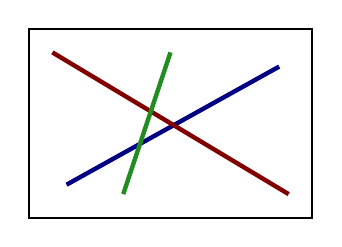
\begin{tikzpicture}[scale = .6]
\draw[thick] (0,0) rectangle (6,4);
\draw[ultra thick, NavyBlue] (.8,.7) -- (5.3,3.2);    
\draw[ultra thick, Maroon] (.5,3.5) -- (5.5,.5);     
\draw[ultra thick, ForestGreen] (2,.5) -- (3,3.5);   
\end{tikzpicture}
\quad \quad 
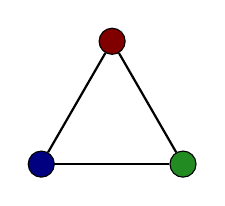
\begin{tikzpicture}[scale = .6]
\node[draw, circle, fill=NavyBlue, minimum size=2mm] (A) at (0,0) {};
\node[draw, circle, fill=ForestGreen, minimum size=2mm] (B) at (3,0) {};
\node[draw, circle, fill=Maroon, minimum size=2mm] (C) at (1.5,2.6) {};

% Draw edges between the vertices
\draw[thick] (A) -- (B);
\draw[thick] (B) -- (C);
\draw[thick] (C) -- (A);
\end{tikzpicture}
\caption{Left: A toy drawing of $X=\PP^{2}\setminus\{\ell_{R},\ell_{B},\ell_{G}\}$. Right: The boundary complex $\Delta(X\subset \overline{X})$ when $\overline{X}=\PP^{2}$.}
\end{figure}
\end{example}


Motivated by the idea that the tropicalization should compute the weight zero compactly supported cohomology this suggests that to construct a tropicalization of a Shimura variety $D/\Gamma$ we wish to find a ``nice'' compactification of $D/\Gamma$ and describe the boundary complex of this compactification. Towards this, I hope to utilize the theory of toroidal compactification to construct tropicalizations of Shimura varieties.

Ash, Mumford, Rapoport, and Tai use the theory of toroidal embeddings and Siegel domains to construct toroidal compactifications of Shimura varieties, that is compactification $D/\Gamma\subset \overline{D/\Gamma}$ such that locally it looks like a torus inside of a toric variety. At extremely high level their approach is to consider the Satake compactification of $D/\Gamma$ (itself not necessarily algebraic) and then at each boundary component $F$ of this compactification glue in toric varieties coming from a polyhedral decomposition of a self-adjoint homogenous cone $C(F)$ one can associate to $F$ module the action of the stabilizer $\Gamma_{F}$ of $F$ and the action of $\Gamma$. As hinted at their construction relies on the additional data of ``a polyhedral decomposition of a self-adjoint homogenous cone $C(F)$'' for each boundary component $F$, they package this data in what is called a $\Gamma$-admissible decomposition.

\begin{defn}
A $\Gamma$-admissible decomposition $\Sigma=\{\Sigma_{F}\}$ is a collection of set $\Sigma_{F}$ one for each rational boundary component $F$ of $D$ such that $\Sigma_{F}=\{\sigma\}$ is an (infinite) collection of rational polyhedral cones in $C(F)$ such that:
\begin{enumerate}
\item the cones in $\Sigma_{F}$ cover $C(F)$,
\item if $\sigma,\sigma\in \Sigma_{F}$ then $\sigma\cap \sigma'$ is a face of both $\sigma$ and $\sigma'$,
\item if $\sigma \in \Sigma_{F}$ and and $\tau \subset \sigma$ is a face then $\tau\in \Sigma_{F}$, and
\item there is an action of $\Gamma_{F}$ on $\Sigma_{F}$ with only finitely many orbits. 
\end{enumerate}
\end{defn}

From this description of a toroidal compactification, we conjecture we are able to construct tropicalizations of Shimura varieties. In particular, for each rational boundary component $F$ we have a group $\Gamma_F$ and a convex cone $C(F)$, we decompose the $C(F)$ into polyhedral cones with finitely many $\Gamma_F$ orbits and then glue the $C(F)/\Gamma_{F}$ together modulo the action of $\Gamma$ on the boundary components. Put imprecisely if $\Sigma=\{\Sigma_{F}\}$ is a $\Gamma$-admissible decomposition then
\[
\left(D/\Gamma\right)^{\Trop,\Sigma} =\bigcup_{\substack{\text{$F$ rational boundary}\\ \text{ component $D$}}} \left(\bigcup_{\sigma \in \Sigma_{F}} \sigma\big/ \Gamma_{F}\right)\big/\Gamma.
\]
A goal of this project is to make the above construction precise and prove the following conjecture. 

\begin{conj}\label{con:main}
    With set-up as above, if $\Sigma=\{\Sigma_{F}\}$ is a $\Gamma$-admissible collection of $D/\Gamma$ then there exists a topological space $(D/\Gamma)^{\Trop,\Sigma}$ with the following properties:
    \begin{enumerate}
    	\item The choice of $\Sigma$ endows $(D/\Gamma)^{\Trop, \Sigma}$ with the structure of a generalized cone complex:
	\[
	\left(D/\Gamma\right)^{\Trop,\Sigma}=\lim_{F}\lim_{\sigma \in \Sigma_{F}} \sigma.
	\]
    	\item Up to homeomorphism $(D/\Gamma)^{\Trop,\Sigma}$ is independent of the choice of $\Sigma$.
	\item For all For all $k\geq0$ there exists natural isomorphisms:
	\[
        H_{k}\left((D/\Gamma)^{\Trop,\Sigma}; \QQ\right) \cong W_{0}H_{c}^{k}\left(D/\Gamma;\QQ\right).
        \]
        \end{enumerate}
\end{conj}

% Now we are ready to encounter our monster. As in a well-arranged science fiction movie, the reader has awaited its apparition on the screen 
In light of part (2) of Conjecture~\ref{con:main} we will often refer to \emph{the} tropicalization of $D/\Gamma$ without reference to the $\Gamma$-admissible decomposition. In many ways Conjecture~\ref{con:main} follows by directly combining the works of of Ash, Mumford, Rapoport, and Tai \cite{AMRT} and  \cite{Deligne71,Deligne74,CGP21} and has been floating in the literature in various ways \cite{harris14,harrisZucker}, however, in ongoing work with collaborators we hope to make this clear and have a tentative proof of Conjecture~\ref{con:main}. Out of an abundance of caution -- and some lingering issues around extending \cite{AMRT} to stacks we are working to resolve -- I only claim it as a conjecture. However, we have carefully verified Conjecture~\ref{con:main} for the mains examples from the previous section: $\cA_{g}$ and $\cA_{g}(m)$ (see Example~\ref{ex:ag}) and $\cA_{p,q,\psi}$ (see Example~\ref{ex:apq}).

\begin{remark}
The work of Ash, Mumford, Rapoport, and Tai  on toroidal compactifications has been studied and extended in numerous ways. Of particular, interest for this project Faltings and Chai \cite{faltingsChai} who construct these compactifications for $\cA_{g}$ and $\cA_{g}(m)$ as stacks over $\ZZ$ and $\ZZ[1/m]$ respectively. Further, in \cite{namikawa80} Namikawa gives a careful exposition with numerous details when $D=\HH_{g}$ is the Siegel upper half-plane. 
\end{remark}


\section{Tropical Modular Interpretation}\label{sec:trop-mod}

As described in Section~\ref{sec:gen-trop} the tropicalization of Shimura variety $D/\Gamma$ is simply a topological space with the structure of a cell complex (more precisely a generalized cone complex or $\Delta$-complex \cite{abramovichCaporasoPayne15, CGP21}). In particular, the points of $(D/\Gamma)^{\Trop}$ do not have any intrinsic meaning. However, since $D/\Gamma$ is often a moduli space of varieties that themselves are of interest (elliptic curves, abelian varieties, K3's, etc.) it is natural to ask whether one can give a ``tropical modular'' interpretation of $(D/\Gamma)^{\Trop}$.  We use the term ``tropical modular'' since we do not mean to imply that we give a modular functor which is represented by $(D/\Gamma)^{\Trop}$ as one might in algebraic geometry, instead we mean the slightly vaguer notion of constructing tropical versions of the parameterized objects (tropical elliptic curves, tropical abelian varieties, tropical K3's, tropical etc.) and showing there is a bijection between the points of $(D/\Gamma)^{\Trop}$ and isomorphism classes of tropical objects.

\begin{problem}\label{rp:trop-modular}
Give a tropical modular interpretation of $(D/\Gamma)^{\Trop}$.
\end{problem}

To give a sense of how this goal plays out in practice let us explore the case of $\mathcal{A}_{g}$ where such a tropical modular interpretation is known. A {\em (principally polarized) tropical abelian variety} of dimension $g$ is a pair $A=(L, Q)$, where $L$ is a free abelian group of rank $g$ and $Q$ is a positive semidefinite form on $L_{\RR}\coloneqq L\otimes_{\ZZ}\RR$ with $L$-rational kernel. (By $L$-rational kernel we mean the $\ker(Q)$ has an $\RR$-basis consisting of elements of $\Lambda$. Two tropical abelian varieties $(L,Q)$ and $(L',Q')$ are \emph{isomorphic} if there is an isomorphism $\phi:L \to L'$ taking $Q$ to $Q'$. Since $\Lambda \cong \ZZ^{g}$ every tropical abelian variety of dimension $g$ is isomorphic to one of the form $(\ZZ^{g},Q)$ where $Q \in \PDrt_{g}$. Further, two tropical abelian varieties $(\ZZ^{g},Q)$ and $(\ZZ^{g},Q')$ are isomorphic if and only if there exists $h\in \GL(g,\ZZ)$ such that $Q'=hGh^{t}$.  Thus, the construction of $\mathcal{A}_{g}^{\Trop}$ as (set-theoretically) $\PDrt_g/ \GL(g,\ZZ)$ gives the following tropical modular interpretation of $\mathcal{A}_{g}^{\Trop}$.

\begin{prop}\cite{BMV11}\label{prop:trop-interp-ag}
There is a bijective correspondence between
\[
\begin{tikzcd}
\mathcal{A}_{g}^{\Trop} \arrow[r, leftrightarrow, "\sim"] & \left\{ \begin{matrix} \text{isomorphism classes of} \\
\text{tropical abelian varieties of dim. $g$}
\end{matrix}\right\}
\end{tikzcd}
\]
\end{prop}

This tropical interpretation is particularly useful in \cite{BBCMMW24} as it provides an extremely nice combinatorial subspace arising from the relationship between tropical abelian varieties and regular matroids.

Beyond Proposition~\ref{prop:trop-interp-ag} there do not exist meaningful tropical modular interpretations of the tropical Shimura varieties conjectured in Conjecture~\ref{con:main}. However, there has been interest in tropical K3's, tropical elliptic curves, and other similar objects that may be of interest in this direction.

In ongoing work towards Research Problem~\ref{rp:trop-modular} together with co-authors we have attempted to make give a tropical modular interpretation of $\cA_{g}(m)^{\trop}$ by introducing a notion of tropical abelian varieties with level structure. 

\begin{defn}
Fix positive integers $g,m\geq1$. A {\em tropical (principally polarized) abelian variety of dimension $g$, with level $m$} structure, is a tuple $(\Lambda,J,\iota,Q)$ where:
\begin{enumerate}
\item $\Lambda$ is a free abelian group of rank $2g$,
\item $J:\Lambda\times \Lambda\to \ZZ$ is an alternating $\ZZ$-bilinear form,
\item $\iota:(\Lambda/m\Lambda\to (\ZZ/m\ZZ)^{2g}$ an isomorphism that takes $J$ to the standard symplectic paring, and
\item $Q:\Lambda_{\RR}\times\Lambda_{\RR}\to \RR$ is a positive semidefinite form whose kernel is $W^{\perp}$ for some $\Lambda$-rational isotropic (with respect to $J$) subspace $W\subset \Lambda_{\RR}$. 
\end{enumerate}
\end{defn}

When $m=1$ this definition reduces to the original definition of a tropical abelian variety given above by taking $(\Lambda, J,\iota,Q)$ to $(\Lambda/\Lambda\cap W', Q)$ where $W'\subset \Lambda_{\RR}$ is any maximal isotropic subspace extending $W$. This leads myself and co-authors to make the following conjectural description of $\mathcal{A}_{g}^{\Trop}(m)$ as a tropical moduli space, which we know to be true when $m=1$ (see Proposition~\ref{prop:trop-interp-ag}) and $m=2$. 

\begin{conj}
There is a bijective correspondence between
\[
\begin{tikzcd}
\mathcal{A}_{g}(m)^{\Trop} \arrow[r, leftrightarrow, "\sim"] & \left\{ \begin{matrix} \text{isomorphism classes of} \\
\text{tropical abelian varieties of dim. $g$}\\
\text{with level structure $m$}
\end{matrix}\right\}
\end{tikzcd}
\]
\end{conj}


As an indication of the usefulness of having a tropical modular interpretation, we note the following beautiful result of Chan, Galatius, and Payne showing that in some sense $\cM_{g}^{\trop}$ realizes the weight zero compactly supported cohomology of $\cM_{g}$.

\begin{theorem}\cite[Section 7]{CGP21} \label{thm:cpg-lambda}
There is a continuous proper map of topological spaces $\lambda: \mathcal{M}_{g}(\CC)\to \mathcal{M}_{g}^{\Trop}$ such that the induced map on compactly supported cohomology naturally factors
\[
\begin{tikzcd}[row sep = 3em, column sep = 3em]
H_{c}^{k}( \mathcal{M}_{g}^{\Trop}; \QQ) \arrow[r, "\lambda_{*}"] \arrow[dr, two heads,dashed] & H^{k}_{c}(\mathcal{M}_{g}; \QQ) \\
& W_{0}H^{k}_{c}(\mathcal{M}_{g}; \QQ) \arrow[u, hook]
\end{tikzcd}
\]
\end{theorem}

The proof of Theorem~\ref{thm:cpg-lambda} is based upon ideas from hyperbolic geometry: one may obtain a dual graph from a Riemann surface by collapsing geodesics that are sufficiently short. And so a priori it is not clear that this should generalize, however, using appropriate tropical modular interpretations I hope to address the following question. 


\begin{problem}\label{rp:lambda}
Using the tropical modular interpretation given in Research Problem~\ref{rp:trop-modular} give a continuous proper map of topological spaces $\lambda:(D/\Gamma)(\CC)\to(D/\Gamma)^{\Trop}$ such that that the induced map on compactly supported cohomology naturally factors
\[
\begin{tikzcd}[row sep = 3em, column sep = 3em]
H_{c}^{k}( (D/\Gamma)^{\Trop}; \QQ) \arrow[r, "\lambda_{*}"] \arrow[dr, two heads,dashed] & H^{k}_{c}(D/\Gamma; \QQ) \\
& W_{0}H^{k}_{c}(D/\Gamma; \QQ) \arrow[u, hook]
\end{tikzcd}
\]
\end{problem}

I have been looking at Research Problem~\ref{rp:lambda} in the setting of $\cA_{g}$, where I note the very partial result. 

\begin{lemma}\label{lem:eps}
Suppose $\Lambda \subset \CC^{g}$ is a lattice of rank $2g$ and $H:\CC^{g}\times \CC^{g}\to \CC$ Riemann form such that $E=\text{Im}(H)$ is integral on $\Lambda$. If $\varepsilon$ is sufficiently small then the real vector space $W_{\epsilon}\coloneqq \RR\langle x\in \Lambda | H(x,x)< \varepsilon\rangle$ is isotropic with respect to $E$.
\end{lemma}

Thus, we may hope to construct a map $\lambda:\cA_{g}\to A_{g}^{\trop}$ by sending a principally polarized abelian variety $(\CC^{g}/\Lambda,H)$ to the tropical abelian variety $(W_{\varepsilon}\cap \Lambda, E)$. Of course, one must also show that this map is well-defined and independent of the choice of $\varepsilon$ (which seems easy), however, checking that it has the desired properties in Research Problem~\ref{rp:lambda} is significantly more subtle, and would be a goal of this proposal. 

One may hope that Theorem~\ref{thm:cpg-lambda} and Research Problem~\ref{rp:lambda} are perhaps an instance of a much more general phenomena about dual complexes and weight-zero compactly supported cohomology.

\begin{question}\label{ques:hodge}
Let $\cX$ be a smooth DM stack and $\cX(\CC)\subset \overline{\cX}$ be a compactification with normal crossings. Does there exist a continuous proper map $\lambda:\cX\to \Delta(\cX \subset \overline{\cX})$ that realizes the weight-zero compactly supported cohomology of $\cX$?
\end{question}

Understanding the answer to Question~\ref{ques:hodge} will likely require a deeper understanding of Deligne's original construction of the weight filtration on a smooth variety $X$ in terms of a smooth normal crossings compactification $X\subset \overline{X}$ and logarithmic de Rham cohomology \cite{Deligne71, Deligne74}.

\begin{remark}
Note that there exists similar comparison results in the literature between tropical and classical moduli spaces, however, they often have a non-archimedean perspective that is different in spirit from Research Question~\ref{rp:lambda}. For example, in \cite{viviani13} Viviani proves that if $K$ is a non-archimedean valued field then there is a commutative diagram of continuous maps
\[
\begin{tikzcd}
\cM_{g}(K) \arrow[r, "\trop"] \arrow[d] & \cM_{g}^{\Trop} \arrow[d]\\
\cA_{g}(K) \arrow[r, "\trop"] & \cA_{g}^{\Trop} 
\end{tikzcd}
\]
where the horizontal arrows Viviani constructs and the vertical maps are the Torelli and tropical Torelli maps. It is not clear how this construct is related to that in \cite[Section 7]{CGP21} or proposed by Lemma~\ref{lem:eps}. However, it would be a further research goal to see if these two perspectives could be put into a broader unifying framework. 
\end{remark}

 

\section{Computing Weight Zero Compactly Supported Cohomology of Shimura Varieties }\label{sec:computing}

While Conjecture~\ref{con:main} provides a theoretical description of the weight zero compactly supported cohomology of a Shimura variety $D/\Gamma$ in terms of the homology of $(D/\Gamma)^{\Trop}$ it would also be interesting to explicitly compute these cohomology groups at least in small dimensions.

\begin{problem}\label{rp:compute}
Explicitly compute the weight zero compactly supported cohomology of $D/\Gamma$ for examples where $D/\Gamma$ has small dimension.
\end{problem}

Note that my work in \cite{BBCMMW24} can be viewed as an answer to this Research Problem~\ref{rp:compute} when $D/\Gamma=\cA_{g}$ as we compute the top weight cohomology (and hence weight zero compactly supported cohomology) for $g\leq 7$ and provide vanishing results for $8\leq g\leq 10$. 

In order to move from the abstract description in Conjecture~\ref{con:main} to explicit computations of cohomology groups we must first find a $\Gamma$-admissible decomposition for which we can describe $(D/\Gamma)^{\Trop,\Sigma}$ (or the associated cellular chain complex) explicitly. In general, this seems  difficult, however, recently coauthors and I have made progress in this direction for $\cA_{2}(m)$. In this setting the cones $C(F)$ can be taken to be the cone $\PDrt_{k}$ of positive semi-definite forms on $\RR^{k}$ with rational kernel. The groups $\Gamma_{F}$ are then $\GL(k,\ZZ)(m)$, and there is a particularly nice admissible decomposition (the perfect cone decomposition) we can work with. Using this we show that  $\cA_2(m)^{\Trop}$ is obtained from $\frac{m^4 - 1}{2}$ $\PDrt_{1}$, and $\frac{m^4 - 1}{2}$ copies of $\PDrt_{2}/\GL(2,\ZZ)(m)$ glued along common rays. Noting that the link of $\PDrt_{2}/\GL(2,\ZZ)(m)$s is homeomorphic to an orientable surface and understanding how these cones are glued we prove the following proposition.

\begin{figure}[H]
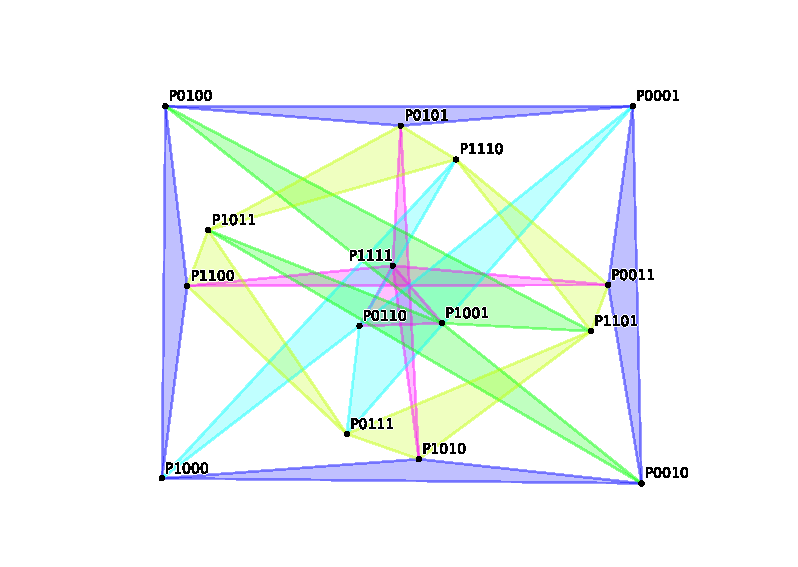
\includegraphics[scale=.6]{A22.pdf}
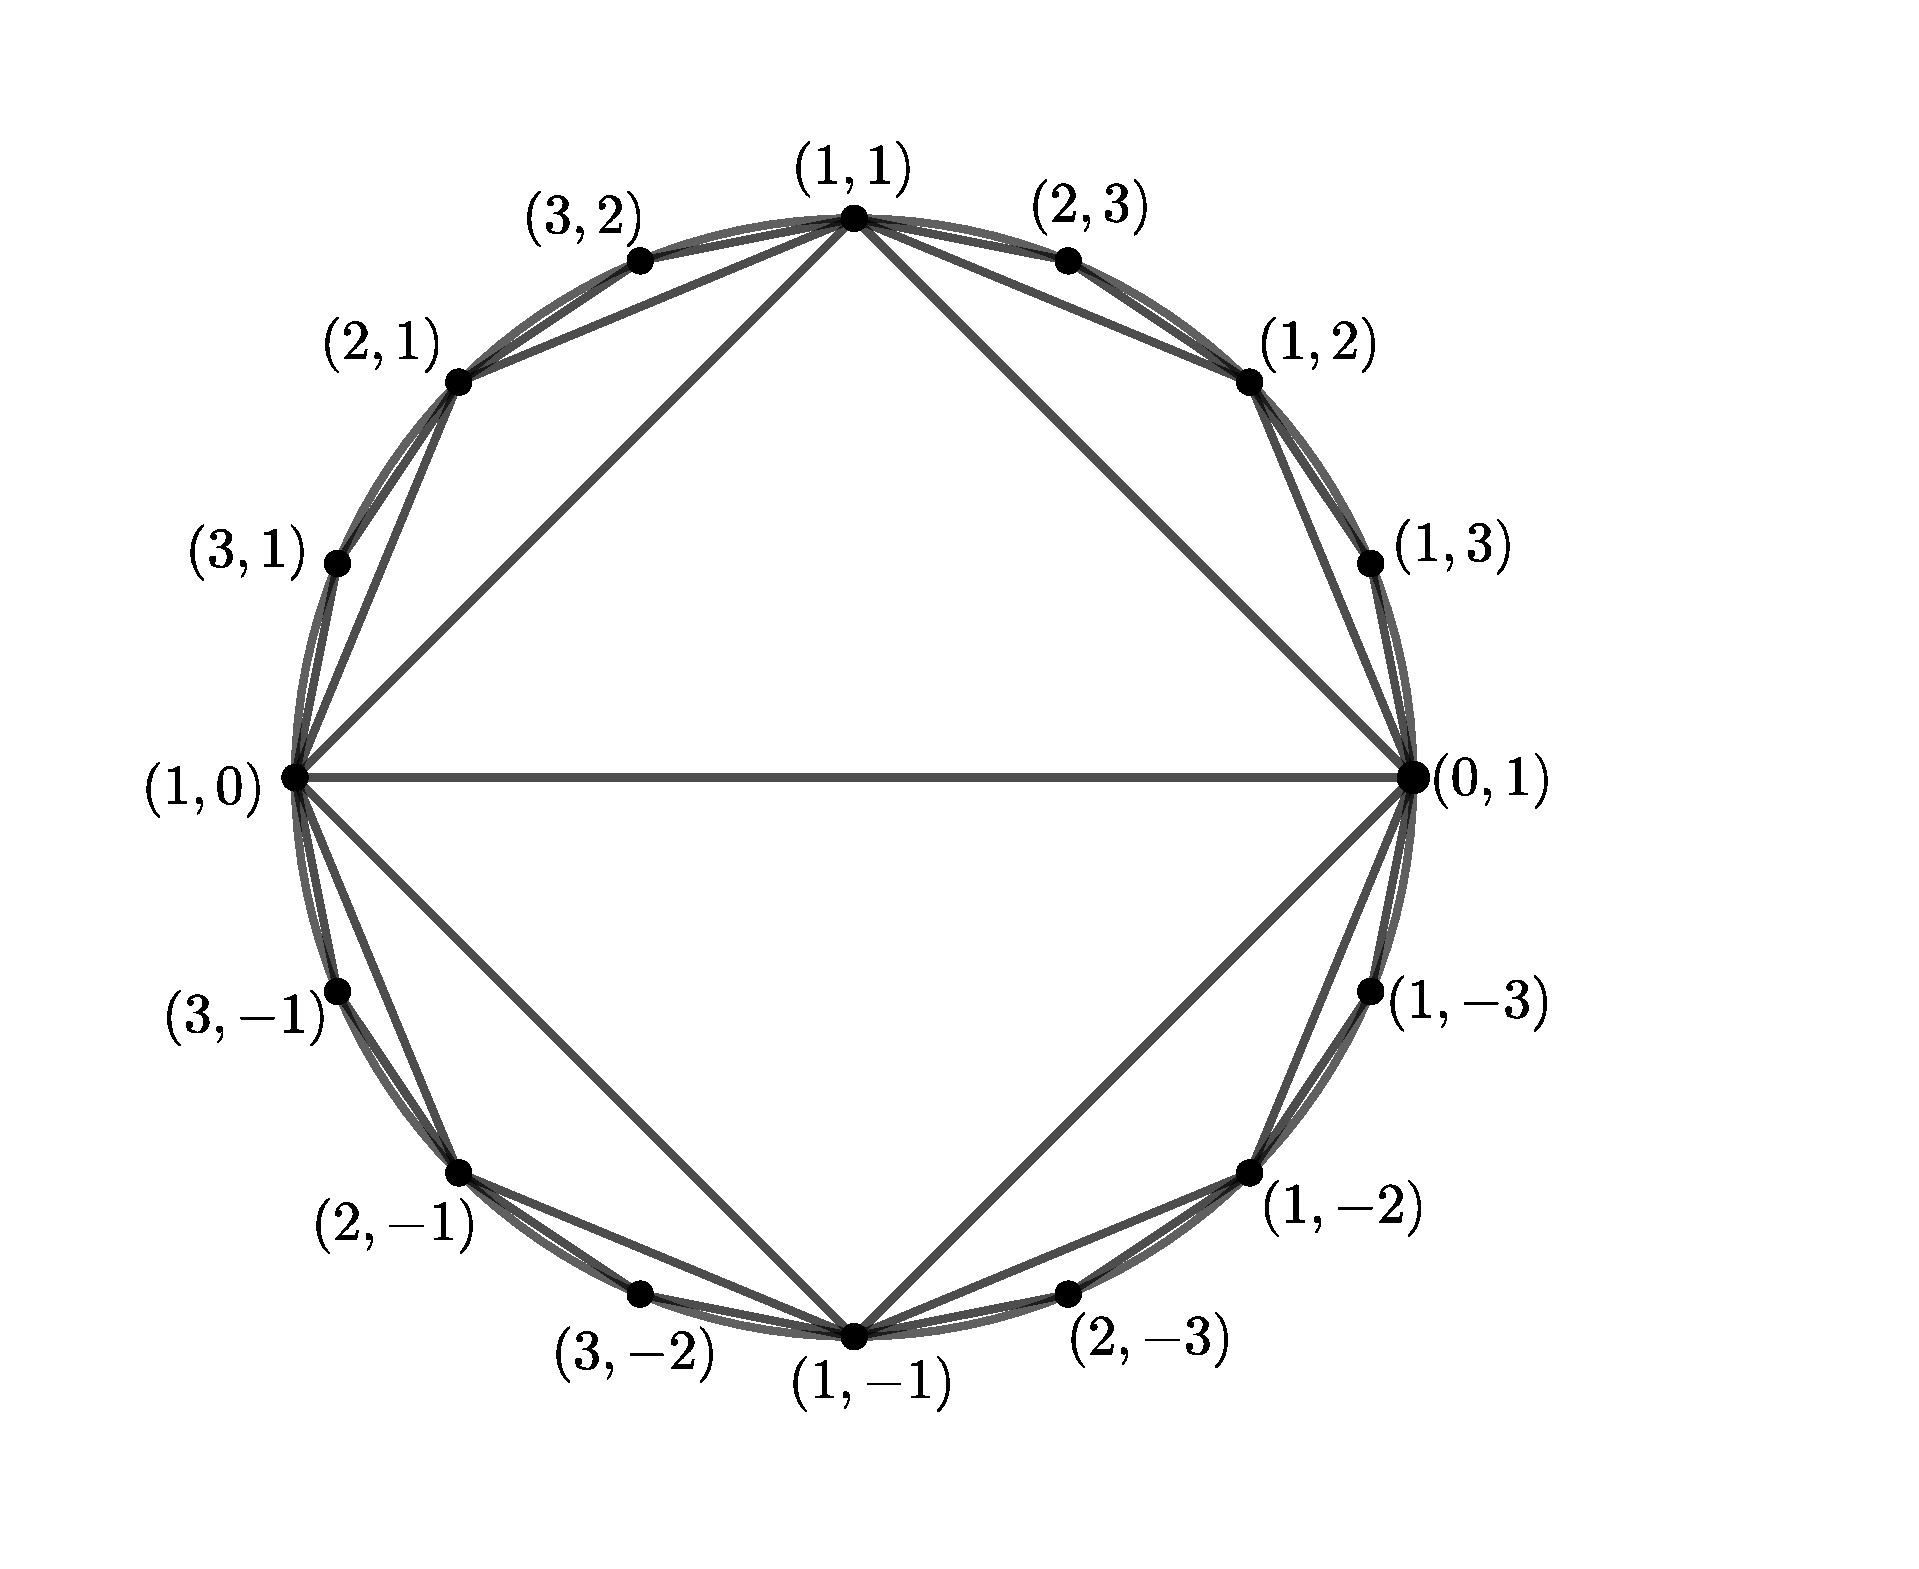
\includegraphics[scale=.195]{perf.pdf}
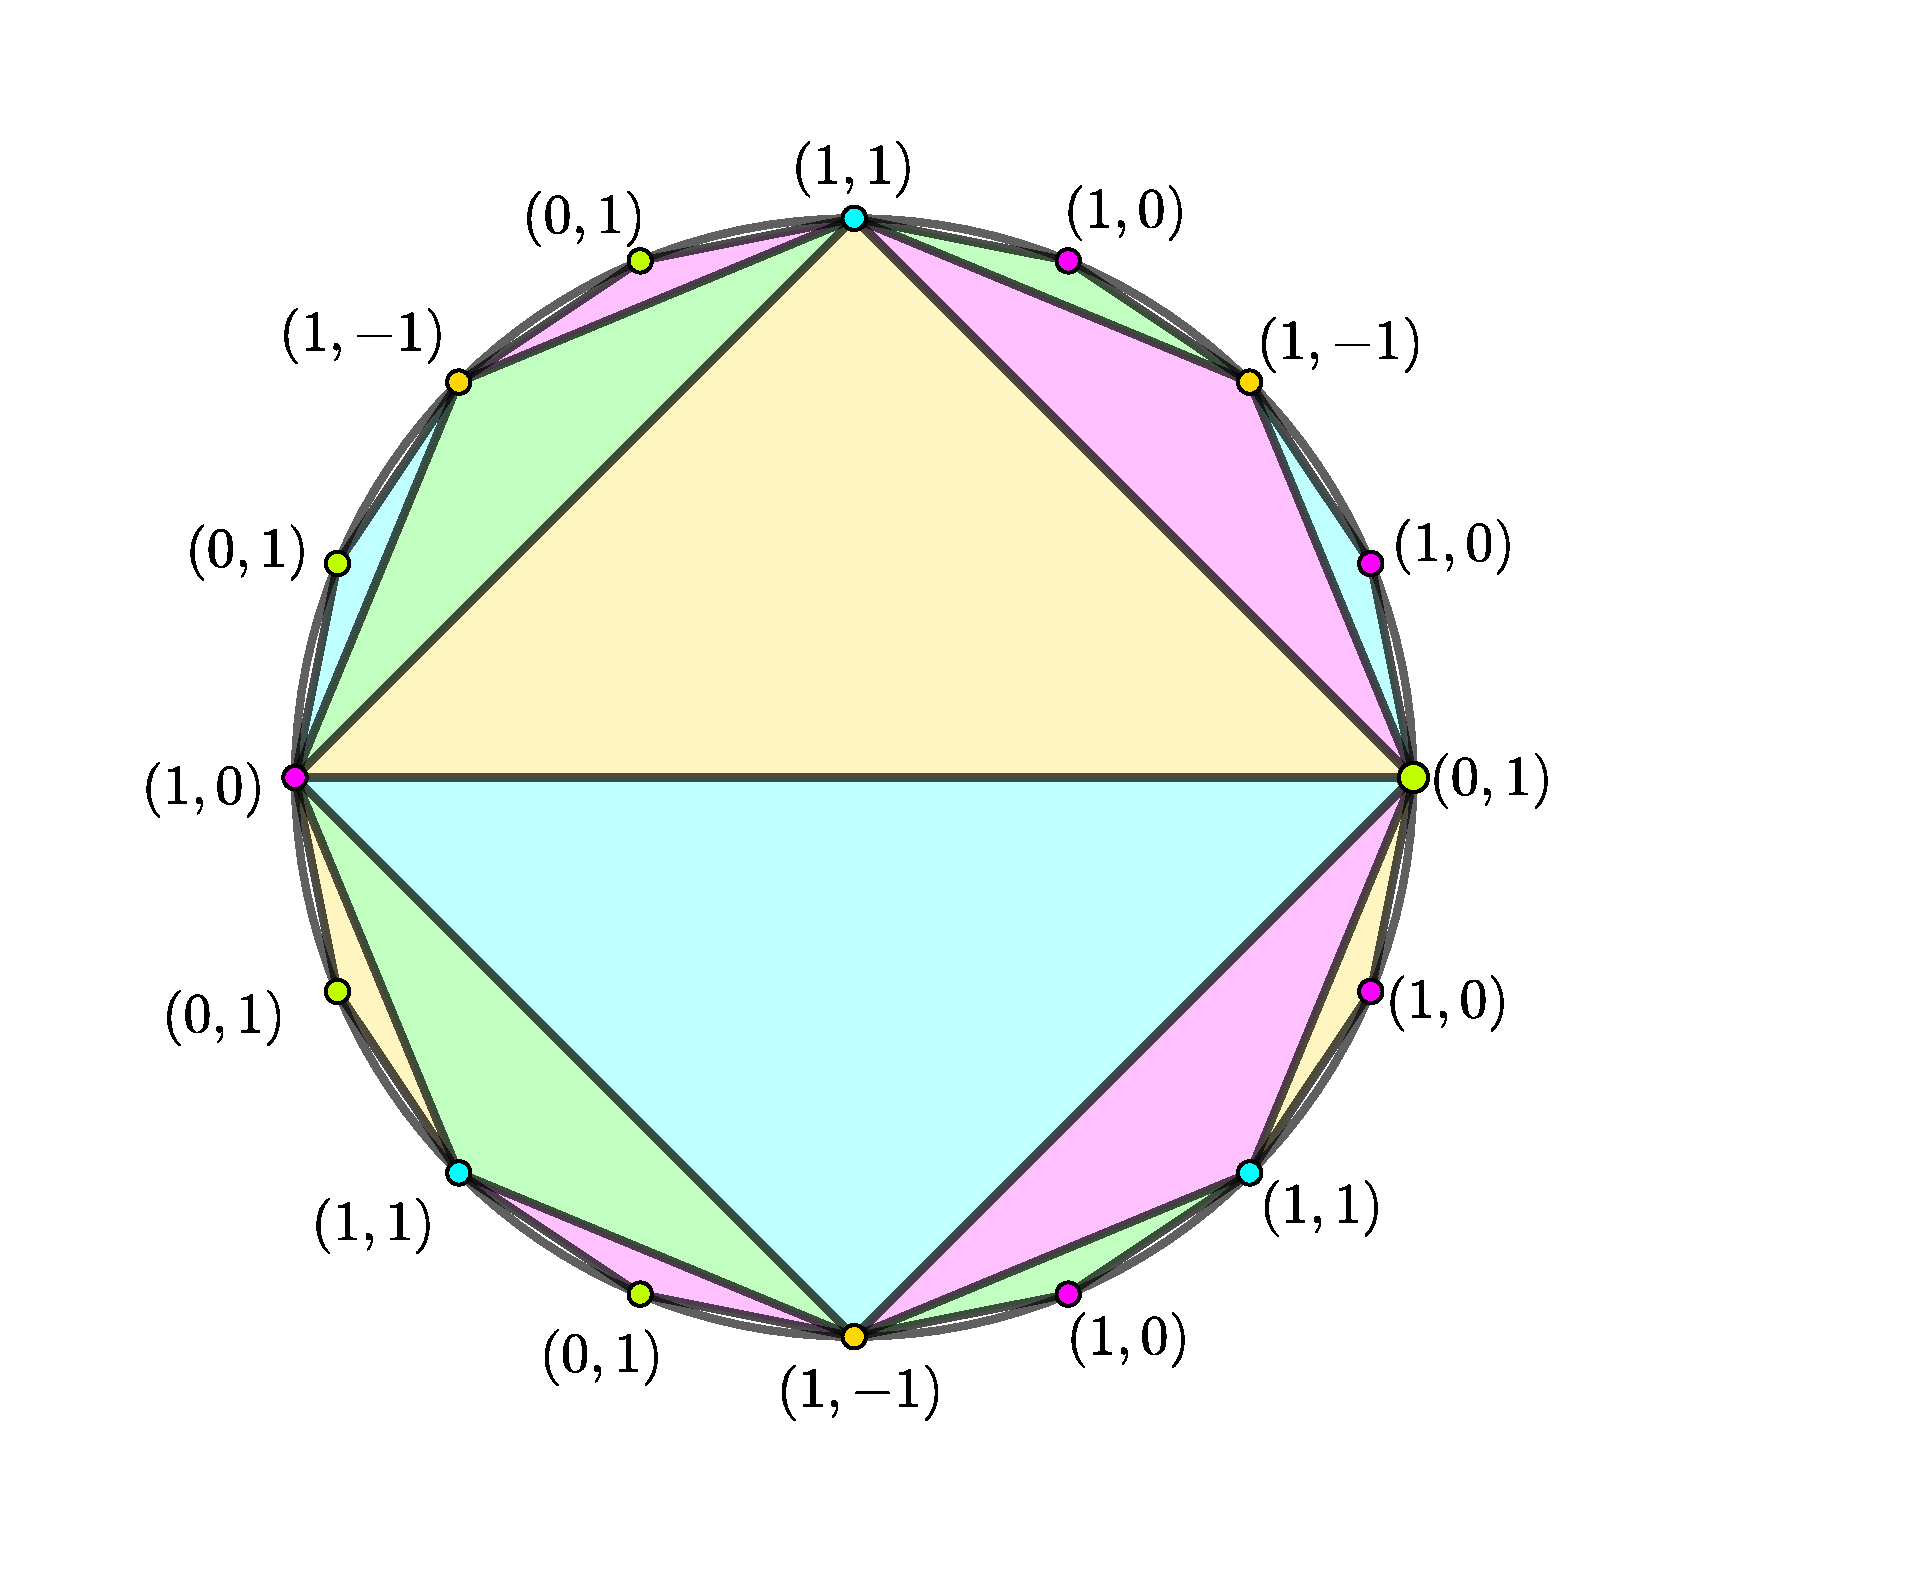
\includegraphics[scale=.195]{perf_3.pdf}
\caption{Left: A picture of $\cA_{2}[2]^{\Trop}$ with vertices labeled by the 15 non-zero vectors in $\FF_{2}^{4}$. Center: A picture of the link of the $\GL(2,\ZZ)$-admissible decomposition of $\PDrt_{2}$. Right: A picture of the action of $\GL(2, \ZZ)(3)$ on the admissible decomposition of $\PDrt_{2}$ given in the center.}
\end{figure}

\begin{prop}\label{prop:a2m}
    Let $m>2$ be a prime number. The weight zero compactly supported cohomology of $\cA_2(m)$ is zero except in the following instances
    \begin{align*}
     W_0 H^2_c(\cA_2(m);\QQ) &= \QQ^{1+ \frac{1}{24} \cdot (m^4-1)(m^3-m)} \\
     W_0 H^3_c(\cA_2(m);\QQ) &= \QQ^{\frac{m^4-1}{2}}. 
    \end{align*}
\end{prop}

Proposition~\ref{prop:a2m} agrees with prior results of Oda and Schwermer who computed the top weight cohomology of $\cA_{2}(m)$ via a Leray spectral sequence argument using Igusa compactifications \cite[Propositions 5.3 and 5.5]{odaSchwermer90}. This proposition gives me hope in tackling the following research questions, which are specific cases of Research Problem~\ref{rp:compute}.

\begin{problem}\label{rp:a2m}
Explicitly compute the weight zero compactly supported cohomology of $\cA_{2}(m)$ for all $m$.
\end{problem}

\begin{problem}\label{rp:computing-computer}
Compute the weight zero compactly supported cohomology of $\cA_{g}(m)$ for all $g\leq 7$ and either all $m$ or all $m\leq 20$.
\end{problem}

We can give a fairly explicit description of a chain complex computing $H_{i}(\cA_{g}(m);\QQ)$ in terms of $\PDrt_{g}/\GL(g,\ZZ)(m)$ and isotropic subspaces of a vector space over a finite field. Thus, answering Research Problems~\ref{rp:a2m} and \ref{rp:computing-computer} reduces to figuring out how to compute the homology of this chain complex. This chain complex is quite complicated, but also rich in structure. I am thus hopeful that it will be possible to develop software for Macaulay2 to generate this chain complex and answer the weak version of Research Problem~\ref{rp:computing-computer}. I feel like this would make an excellent senior thesis for the undergraduate I am currently mentoring.

I end this section on a highly speculative question that the computations discussed in this section led Peter Sarnak to ask in personal communications. 

\begin{question}
What is the relationship between the weight zero compactly supported cohomology of $\cA_{g}(m)$ and Siegel Eisenstein series?
\end{question}

Roughly since the weight zero compactly supported cohomology of $\cA_{g}(m)$ comes from understanding the boundary of a locally symmetric space, one may hope it is related to Siegel–Eisenstein series. Some work in this direction has been done in \cite{harrisZucker,harris14}. However, I hope that the methods and computations developed in this proposal should shed new light on answering it. 


\section{Algebraic Structures on the Cohomology of Shimura Varieties}\label{sec:alg-structure}

As hinted at in Section~\ref{sec:trop-moduli} a key step in moving beyond constructing individual non-trivial cohomology classes to proving exponential lower bounds on the dimension of cohomology groups of $\cM_{g}$ is the fact $\oplus_{g} W_{0}H_{c}^{k}(\cM_{g};\QQ)$ has additional algebraic structure (namely a large free sub-Lie algebra). Inspired in part by conjectures in my prior work \cite{BBCMMW24} recently Brown, Chan, Galatius, and Payne have shown that a similar (but more complicated) story occurs of $\cA_{g}$.

\begin{theorem}\cite[Theorem 1.1]{BCGP24}
Let $\cA\coloneqq \sqcup_{g\geq0}\cA_{g}$ be the disjoint union of the moduli principally polarized abelian varieties of dimension $g$ for all $g\geq0$. The weight zero compactly supported cohomology $W_{0}H^{\bullet}_{c}(\cA;\QQ)=\oplus_{k} W_{0}H^{k}(\cA;\QQ)$ has a bigraded Hopf algebra structure.\end{theorem}

\begin{cor}\cite[Corollary 1.5]{BCGP24}
There are at most 20 values of $k$ for which $\dim_{\QQ} H^{2g+k}_{c}(\cA_{g}; \QQ)$ does not grow at least exponentially in $g$ .
\end{cor}

These results motivate the following general question I hope to address as part of this proposal. 

\begin{problem}\label{rp:inflation}
Are there other families of Shimura varieties for which the weight zero compactly supported cohomology has interesting homological structure?
\end{problem}

In the setting of $\cA_{q,q,\psi}$ co-authors and I are close to providing an affirmative to Research Problem~\ref{rp:inflation} in certain settings. Going forward we let $E$ be an imaginary quadratic extension with class number one and $R$ its ring of integers. The key to doing this is the following general theorem concerning the topicalizations  $\cA_{q,q}^{\Trop}$. 

\begin{theorem}\label{thm:inflation-A-case} 
Then there are injections
\[
\begin{tikzcd}
\cA_{0,0}^{\Trop} \arrow[r, "\iota_{0}"] & \cA_{1,1}^{\Trop} \arrow[r, "\iota_{1}"] &\cA_{2,2}^{\Trop} \arrow[r, "\iota_{2}"] &\cdots;
\end{tikzcd}
\]
with $\cA_{q,q}^{\Trop} \setminus i_{q-1}(\cA_{q-1,q-1}^{\Trop}) \cong \PD^\mathrm{Herm}_q/\GL(q,R)$.  Truncating at $\cA_{q,q}^{\Trop},$ the associated relative homology spectral sequence is therefore
\[E^1_{s,t} = \begin{cases} H^{\mathrm{BM}}_{s+t} (\PD^\mathrm{Herm}_s/\GL(s,R);\QQ) & \text{if }s \le q,\\ 0 & \text{else}\end{cases}\]
which converges to $H_{s+t}^{\mathrm{BM}} (\cA_{q,q}^{\Trop};\QQ).$
\end{theorem}

The proof of Theorem~\ref{thm:inflation-A-case} relies on a detailed understanding of the construction of $\cA_{q,q}^{\Trop}$ and explicitly writing down a way to ``inflate'' a point in  $\cA_{q,q}^{\Trop}$ to a point in $\cA_{q+1,q+1}^{\Trop}$. Based on examples, as well as what occurs in the case of $\cA_{g}$ the spectral sequence in Theorem~\ref{thm:inflation-A-case} seems extremely well behaved, and we conjecture that:

\begin{conj}\label{con:inflation-A-case}
The spectral sequence in Theorem~\ref{thm:inflation-A-case} converges to $0$ on the $E_2$-page.
\end{conj}

Assuming this conjecture by extending the methods of \cite{BCGP24} we are then able to prove the following conditional result. 

\begin{theorem}
Assuming Conjecture~\ref{con:inflation-A-case} there is a Hopf algebra structure on the bigraded vector space $\bigoplus_{k,g} W_0 H^k_c(\cA_{g,g,\psi};\QQ)$
with $ W_0 H^k_c(\cA_{g,g,\psi};\QQ)$ in bidegree $(g,k-g)$.
\end{theorem}

I hope this story can be generalized both to other specific families of Shimura varieties and to a more general statement about the existence of a relative homology spectral sequence and the obstructions to its convergence on the $E_{2}$-page. In particular, we have the following conjecture that suggests \cite[Theorem 1.1]{BCGP24} does not generalize in a clear way to $\cA_{g}(m)$ for $m\geq2$.

\begin{conj}
Fix $m\geq2$ there are injections
\[
\begin{tikzcd}
\cA_{0}(m)^{\Trop} \arrow[r, "\iota_{0}"] & \cA_{1}(m)^{\Trop}  \arrow[r, "\iota_{1}"] & \cA_{2}(m)^{\Trop}  \arrow[r, "\iota_{2}"] &\cdots;
\end{tikzcd}
\]
and an associated relative homology spectral sequence
\[E^1_{s,t} = \begin{cases} H^{\mathrm{BM}}_{s+t} (\PD^\mathrm{Herm}_s/\GL_s(R);\QQ) & \text{if }s \le q,\\ 0 & \text{else}\end{cases}\]
which converges to $H_{s+t}^{\mathrm{BM}} (\cA_{q,q}^{\Trop};\QQ)$ but not on the $E_2$-page. 
\end{conj} 

\section{Broader Impacts}\label{sec:broader-impacts} 

\subsection{Organizing} As discussed previously, I have organized 10+ national/international conferences, and I plan to continue organizing conferences at roughly this pace. Currently, I am organizing two research conferences in algebraic geometry \textit{Algebraic Geometry Northeastern Series (AGNES)} and \textit{BATMOBILE} both occurring in late 2024. I am also in the early stages of organizing an international workshop with Diane Maclagan on multigraded homological algebra and toric geometry, which I hope will occur in 2025. Tyler Kelly, Mike Hill, and I are also in the planning stages of organizing a satellite conference for LGBTQ+ mathematicians for the 2026 ICM in Philadelphia. 


The``GEMS'' workshop series that I co-founded sought to build a diverse community of mathematicians to address gender equity in the mathematical community from new perspectives. In particular, these conferences are indented to supplement the affinity group model of the \textit{Women in...} conference series by promoting broad conversations and networks. Going forward I am interested in expanding these ``GEMS'' workshops to other areas of mathematics and creating cross-field discussions that broaden the standard notion of gender equity in mathematics. In particular, there is a planned follow-up to \textit{GEMS in Commutative Algebra} scheduled for Fall 2025, and I am tentatively planning a version of \textit{GEMS in Algebraic Geometry} for 2026. As more of these conferences occur, I have plans to try to work with mathematicians in other fields to organize their own version of \textit{GEMS in...} conferences in their fields. 

When organizing these conferences I paid particular attention to making them as inclusive of women and non-binary researchers as possible. For example, I designed the registration form to be thoughtful of the concerns of transgender researchers and highlighted the locations of single occupancy and ADA-compliant restrooms. The importance of such efforts was highlighted by the following comment I received from a participant, ``I just wanted to thank you for making this workshop inclusive for people with all gender identifications. ... I have always felt out of place when I participated in conferences/workshops for women when they do not specify that non-binary people are welcome ... I really appreciate those questions you put in the registration form. It means a lot to me.'' I would like to work with various professional societies (AMS, AWM, NAM, Spectra, etc.) and research institutes (SLMath, ICERM, IAS, etc.) to produce a guide of best practices for organizing welcoming and inclusive mathematics conferences. By doing this I hope to make it easier for others to organize welcoming events. 

\subsection{ National \& International Advocacy.} I have worked with the Executive Committee of the \textit{Association for Women in Mathematics} to consider ways they could expand their support of women and non-binary mathematicians. I hope to continue this work and find further ways the AWM can support both women and non-binary mathematicians. Since Winter 2023 I joined SLMath's (formerly MSRI's)  \textit{Committee on Women in Mathematics}. I plan to remain on this committee until 2028 when my term is set to expire. In this role, I am hoping to organize a yearly retreat at SLMath that brings together small groups of 5-8 women (and underrepresented individuals more generally) who have been implementing innovative ideas promoting equity in mathematics and brainstorm ways to scale their efforts and effect radical positive change for women in mathematics.  



\subsection{A More Inclusive Learning Community.}  Going forward I am excited to continue my work supporting LGBTQ+ students, and would love to continue building organizations to do so. In particular, given the amazing successes of programs like MSRI-UP and the EDGE Program, I would love to organize a summer REU program specifically aimed at supporting and promoting LGBTQ+ mathematicians. Further, I am in the early stages of planning a mentorship program to help guide LGBTQ+ undergraduates through the process of applying to graduate programs in mathematics and helping young LGBTQ+ graduate students establish themselves. The plan would be to break participants into groups with each group having LGBTQ+ mathematicians at various career stages, thus allowing participants to exchange advice, find support, and build mentoring networks.

\subsection{Mentoring.} As a new faculty member at Dartmouth College I hope to continue and expand the mentoring I do with students, continuing a focus on mentoring students from underrepresented groups. Since arriving on campus in the late Summer I have begun mentoring one graduate student and one undergraduate woman. While still early it seems likely that I will end up co-advising the graduate student and advising the undergraduate's senior thesis. I am also working with the college's AWM Student Chapter and the Out in STEM Student Chapter. 


\newpage
\renewcommand{\bibliofont}{\normalsize}
%%%%%%%%%%%%%%%%%%%%%%%%%%%%%%%%%%%%%%%%%%%%%%%%%%%%%%%%%%%%%%%%%%%%%%%%%%%%%%%%%%%%%%%%%%%%%%%%%%%%%%%%%%
\bibliographystyle{alpha}
\bibliography{sample}

%%%%%%%%%%%%%%%%%%%%%%%%%%%%%%%%%%%%%%%%%%%%%%%%%%%%%%%%%%%%%%%%%%%%%%%%%%%%%%%%%%%%%%%%%%%%%%%%%%%%%%%%%%

\end{document}